O pr�ximo teste (Tabela \ref{tabela:teste1} e Figura \ref{fig:teste1}) mostra o impacto na mudan�a do n�mero de \emph{octaves}, considerando o n�mero de terrenos vizinhos fixo em 2. Quanto maior o n�mero de \emph{octaves}, maior o n�mero de v�rtices da malha do terreno; explicando assim o FPS menor.

Por causa dessa rela��o entre n�mero de \emph{octaves} e n�mero de v�rtices da malha, � poss�vel fazer, em trabalhos futuros, uma gera��o dos terrenos com um n�mero de \emph{octaves} variando de acordo com a dist�ncia da c�mera.

\begin{figure}[H]
	\center{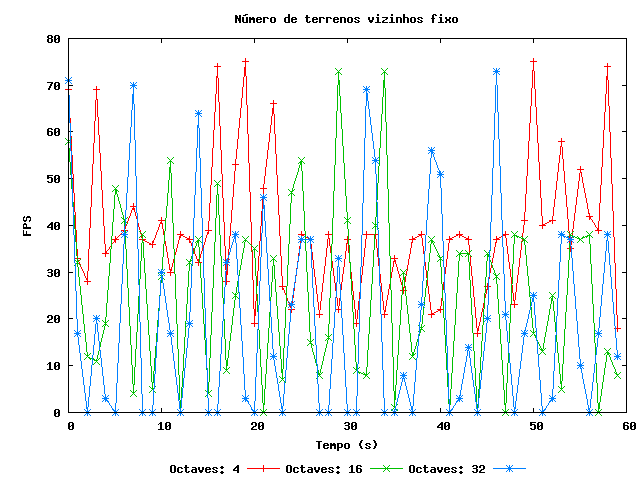
\includegraphics[width=0.8\linewidth]{img/graficos/teste1/teste1.png}}
	\caption{\label{fig:teste1} Teste variando o n�mero de \emph{octaves}, e o n�mero de terrenos vizinhos fixo em 2.}
\end{figure}

\begin{table}[H]
	\begin{center}
		\begin{tabular}{|c|c|c|c|c|}
			\hline
			 - & \multicolumn{3}{|c|}{\emph{Frames} por segundo} \\
			\hline
			 \emph{Octaves} & \scriptsize M�n. & \scriptsize M�x. & \scriptsize M�dia \\
			\hline
			4 & 17,0 & 75,0 & 38,5 \\
			\hline
			16 & 0 & 73,0 & 25,6 \\
			\hline
			32 & 0 & 73,0 & 19,9 \\
			\hline
		\end{tabular}
		\caption{FPS das execu��es variando o n�mero de \emph{octaves}, e o n�mero de terrenos vizinhos fixo em 2.}
		\label{tabela:teste1}
	\end{center}
\end{table}